\documentclass[11pt]{article}
%Gummi|065|=)
\title{Homework \#4: Discussion on Recommender Systems}
\author{Doug McGeehan\\
		CS 6001: Applied Spatial and \\ Temporal Data Analysis\\
		Spring 2017}

\usepackage[margin=1in]{geometry}
\usepackage{verbatim}
\usepackage{framed}
\usepackage{amsmath}
\usepackage{amssymb}
\usepackage{graphicx}
\usepackage{caption}
\usepackage{subcaption}

\begin{document}

\maketitle

\section{Introduction}

Recommender systems provide to a user a score on items they might be interested in.
This score is based on their past ratings and on those of other users.
In this report, five approaches to recommender systems are evaluated on their effectiveness to correctly compute a user's rating.
These approaches can be split into two classes: first, matrix factorization based approaches utilize dimensionality reduction in order to reduce sparsity of the problem; second, collaborative filtering clusters together entities, either users or items, based on similarities in their known ratings.
Here, a user's rating on an entity is based on the weighted sum of ratings from the top-$k$-most similar users or items.

\begin{figure}[h!] \label{fig:somethingelse}
	\centering
	\begin{subfigure}{.5\textwidth}
	  \centering
	  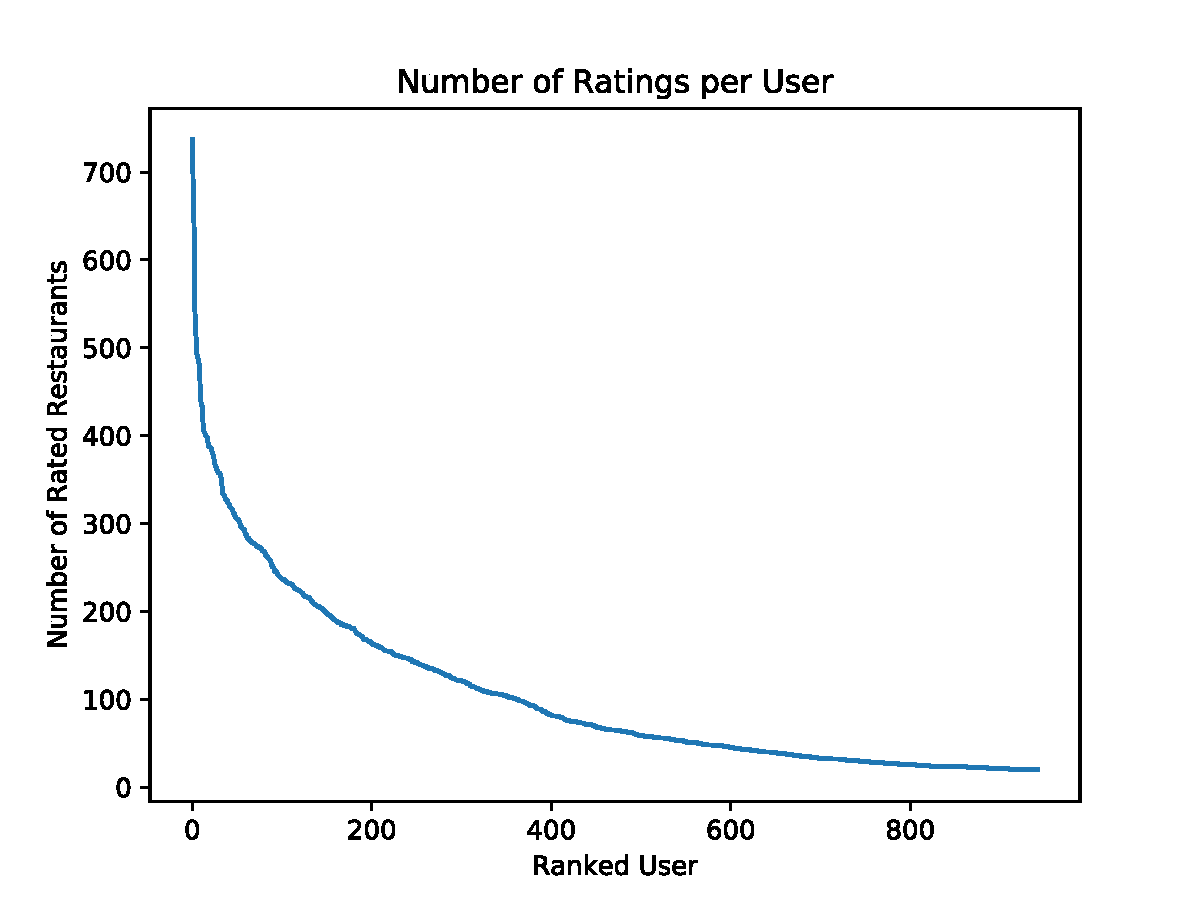
\includegraphics[width=\linewidth]{ratings_per_user}
	  \caption{}
	\end{subfigure}%
	\begin{subfigure}{.5\textwidth}
	  \centering
	  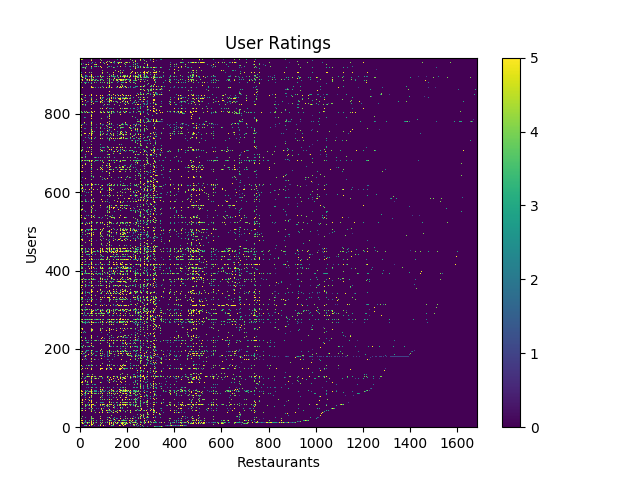
\includegraphics[width=\linewidth]{heatmap}
	  \caption{}
	\end{subfigure}
	\caption{Visualizing the restaurant rating dataset using in this report.}
\end{figure}


These systems are evaluated using a restaurant rating dataset consisting of the ratings from 943 users assigned to a 1,682 restaurants.
These ratings range from 1 to 5.
Figure 1a illustrates the number of restaurants that each user has already rated, exhibiting a power-law distribution where, although it is common to see some users providing many ratings, most users have only provided few.
In Figure 1b, each user's rating of each restaurant is represented as a colormap, with the darkest regions representing absent ratings.
From these two figures, it is evident that this dataset is significantly sparse and imbalanced, and many ratings will need to be estimated by the discussed systems.
To evaluate the effectiveness of these systems, 3-fold cross validation is performed on the dataset.%, and existing ratings in the testing dataset of a particular fold are compared against their estimated ratings from the training dataset.
Mean absolute error (MAE) and the root mean squared error (RMSE) are used for for these comparisons.


\section{Comparing the Five Methods} \label{sec:experiments}

In this section, the performance of five recommender system approaches is evaluated.
Three of these systems approach the problem by using matrix factorization: Singular Value Decomposition (SVD), Probabilistic Matrix Factorization (PMF), and Non-negative Matrix Factorization (NMF).
The remaining two approaches use $k$-nearest neighbors through User-based Collaborative Filtering or Item-based Collaborative Filtering, where a rating on an item is based on the $k$-neighborhood of either users or items, respectively.
The effectiveness of each system is measured using the mean absolute error (MAE) and the root mean squared error (RMSE) between estimated ratings and pre-existing ratings in a 3-fold cross validation on the dataset.


\begin{figure}[h!] \label{fig:threefoldcross}
  \centering
  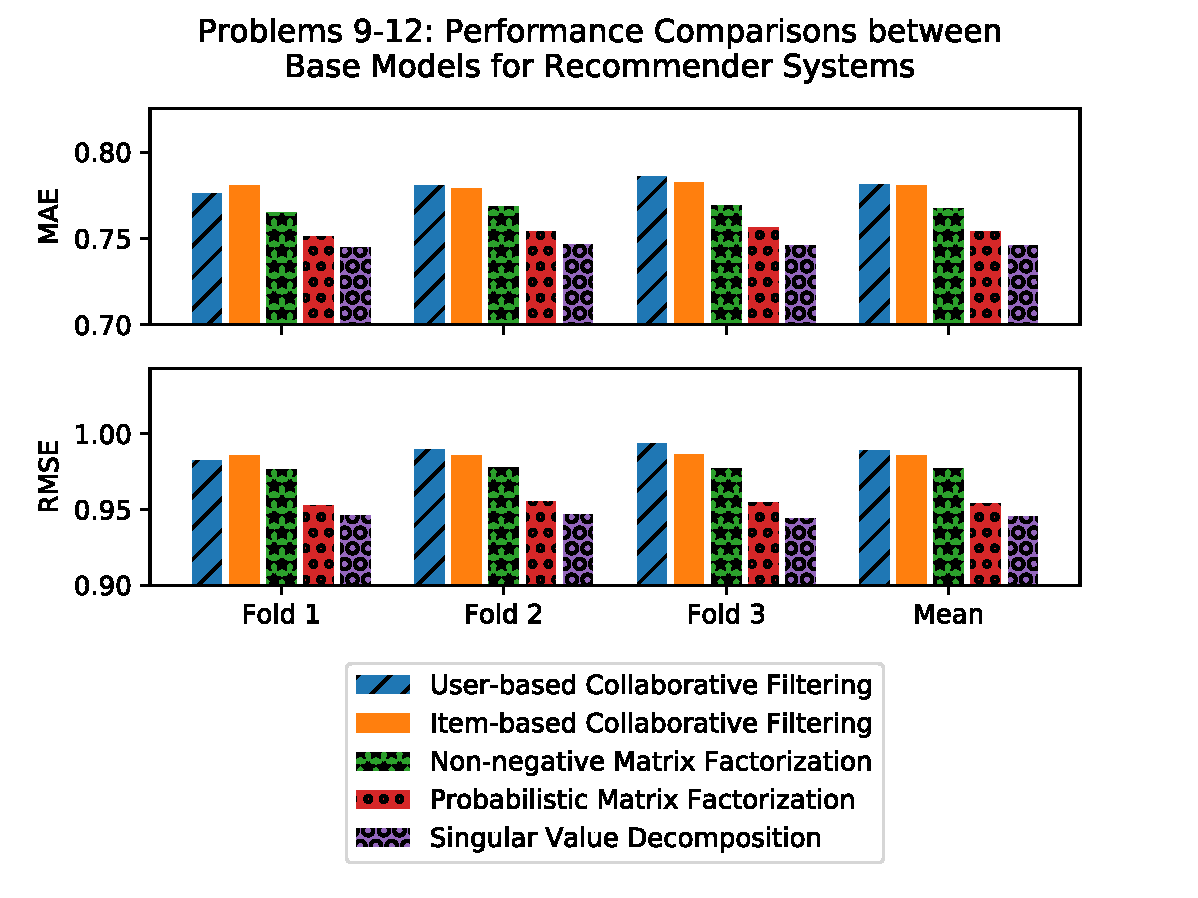
\includegraphics[width=0.8\textwidth]{rmse_mae_comp}
  \caption{}
\end{figure}

From Figure 2, the matrix factorization-based approaches outperformed the $k$NN-based approaches.
This is likely due to the sparsity of the dataset, which remains unhandled in the $k$NN approach but is mitigated through matrix factorization.
The approach with the least error is the Singular Value Decomposition method, with the Probabilistic Matrix Factorization method performs the second best, followed by Non-negative Matrix Factorization.
Both of the collaborative filtering approaches performed the worst, suggesting that the sparsity of the dataset impacted the overall effectiveness of using $k$NN to calculate recommendations.
The Item-based Collaborative Filtering performed only slightly better on average than the User-based approach.
It should be noted, however, that the differences between the measured errors is quite low.
The error of the best-performing method was approximately 5\% below that of the worst performing method.


%\begin{figure}[h!] \label{fig:something}
%  \centering
%  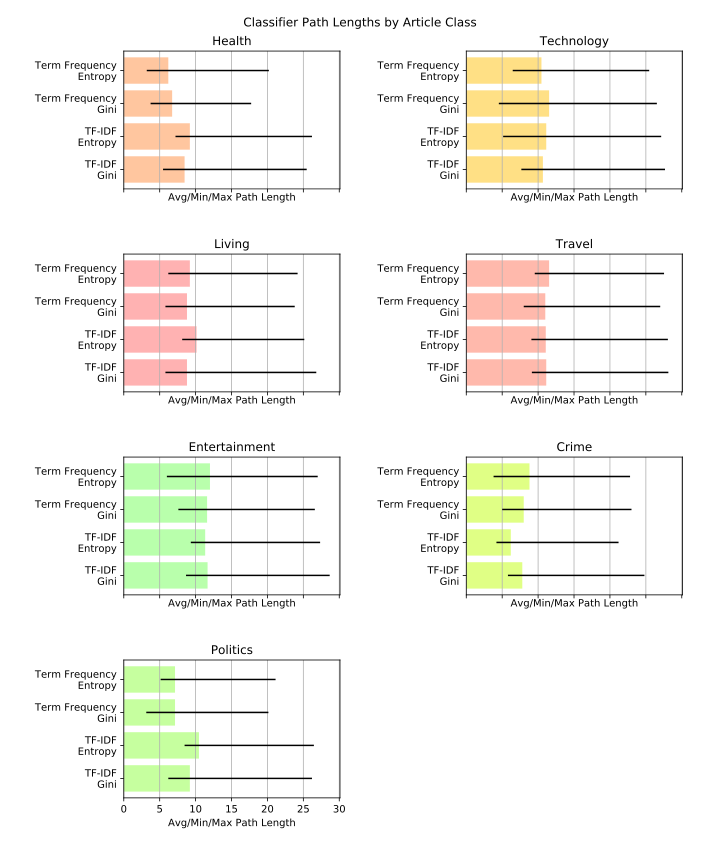
\includegraphics[width=\textwidth]{figures/decision_tree/mrmr/path_depths}
%  \caption{}
%\end{figure}

%\begin{figure}[h!] \label{fig:somethingelse}
%	\centering
%	\begin{subfigure}{.5\textwidth}
%	  \centering
%	  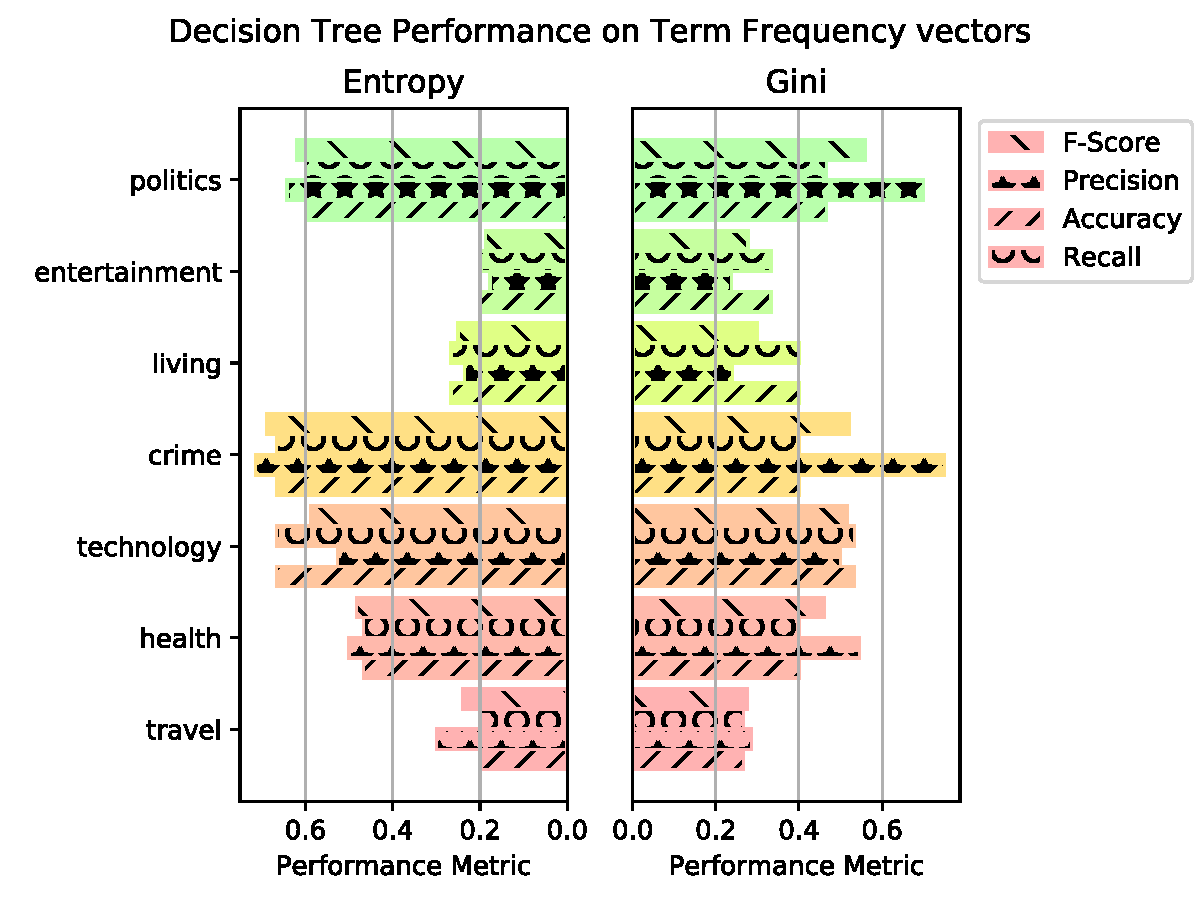
\includegraphics[width=\linewidth]{figures/decision_tree/tf_prec_n_rec}
%	  \caption{}
%	\end{subfigure}%
%	\begin{subfigure}{.5\textwidth}
%	  \centering
%	  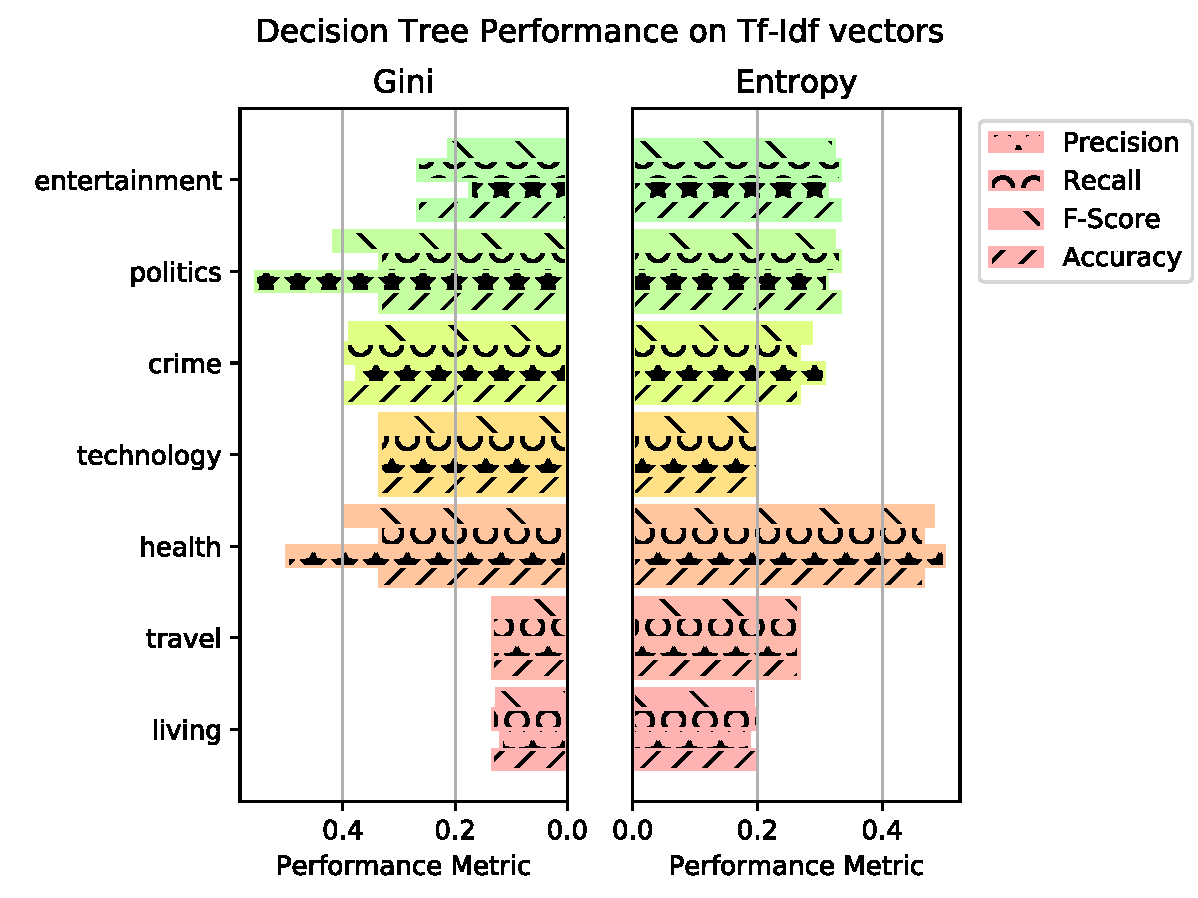
\includegraphics[width=\linewidth]{figures/decision_tree/tfidf_prec_n_rec}
%	  \caption{}
%	\end{subfigure}
%	\caption{}
%\end{figure}

\section{Comparing Similarity Measures for Collaborative Filtering}

Since collaborative filtering is based on $k$NN, its use of a user-specified similarity measure impacts its effectiveness in estimating unknown ratings.
By default, the \texttt{surprise} Python library uses the Mean Squared Differences (MSD) to compute the similarity between a pair of users or a pair of restaurants.
However, it can be configured to use the cosine similarity or the Pearson correlation coefficient.
Figure 3 illustrates the impacts of these measures on the performance of User-based and Item-based collaborative filtering.

\begin{figure}[h!] \label{fig:something}
  \centering
  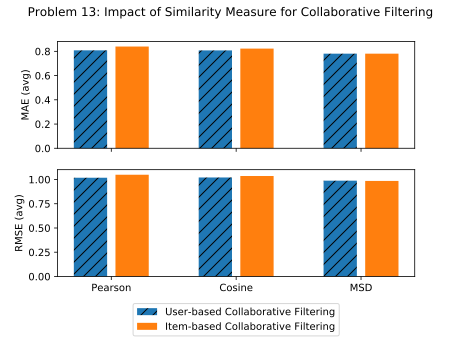
\includegraphics[width=0.8\textwidth]{sim_comp}
  \caption{}
\end{figure}

From Figure 3, it is apparent that the impact of these three similarity measures is consistent for both User-based and Item-based collaborative filtering.
MSD results in both approaches achieving approximately the same error, with Item-based collaborative filtering achieving slightly lower RMSE.
With cosine similarity and the Pearson correlation coefficient, the User-based collaborative filtering performs about 5\% better than Item-based collaborative filtering.
The use of the Pearson correlation coefficient results in the worst performance of Item-based Collaborative filtering, but the performance of User-based Collaborative filtering remains approximately the same in the use of the Pearson correlation coefficient and the cosine distance.


\section{Effect of Neighbor Count on Collaborative Filtering}

Additionally for collaborative filtering, the number of neighbors used to estimate a missing rating will also have an impact on the method's effectiveness.
By default, the \texttt{surprise} Python library uses the 40 nearest neighbors of an item or user to make its estimation.
Figure 4 illustrates the impact on performance when $k$ is varied between 2 and 100.

\begin{figure}[h!] \label{fig:something}
  \centering
  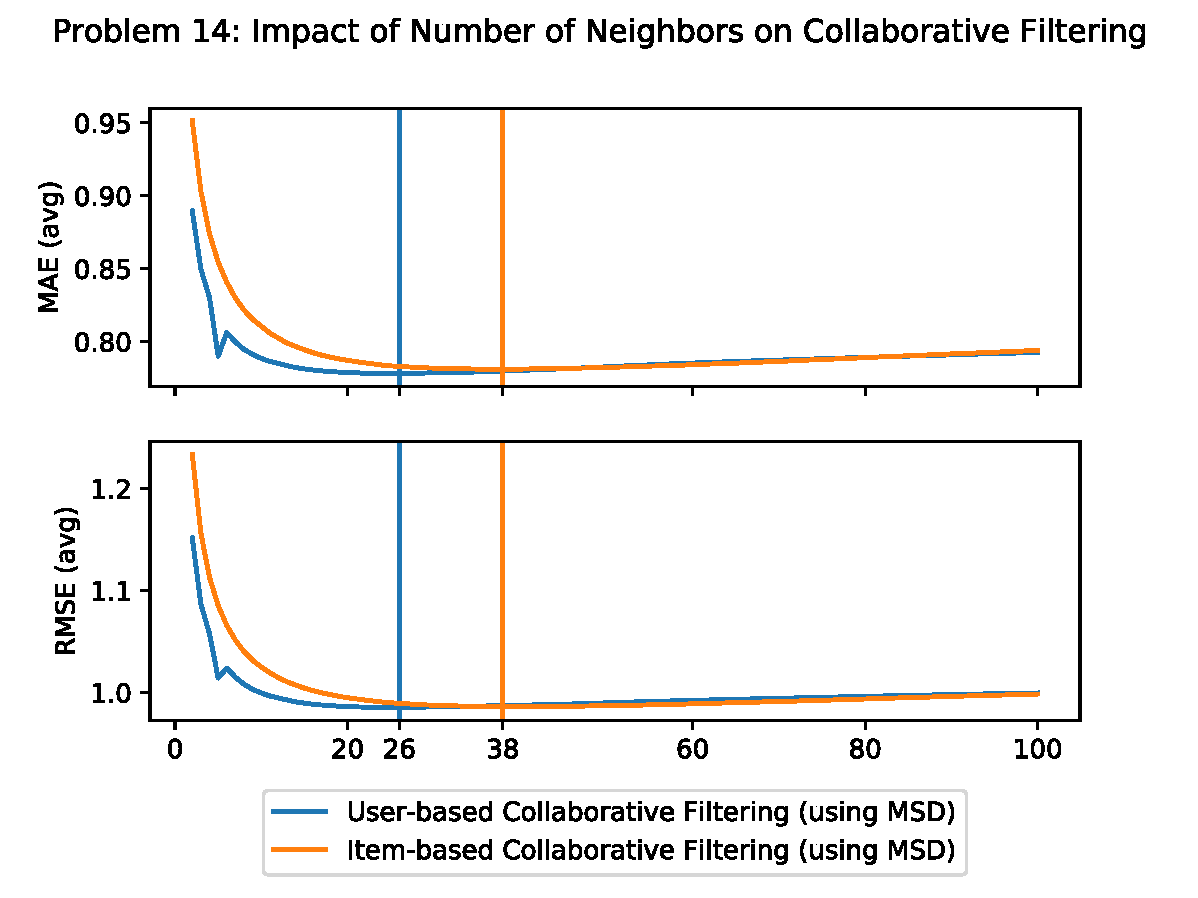
\includegraphics[width=0.8\textwidth]{sim_vark}
  \caption{}
\end{figure}

By averaging the MAE and the RMSE across each execution in a 3-fold cross validation, the best $k$ value for minimizing a method's error is different for each method: User-based collaborative filtering requires 26 neighbors to minimize its error, whereas Item-based collaborative filtering requires 38 neighbors.
Essentially, User-based collaborative filtering is better for fewer neighbors.
In more detail, Item-based collaborative filtering has a slower decline in error as $k$ approaches 38, whereas User-based collaborative filtering reaches its minimum at 26 quite rapidly.
Should execution time be important and a suboptimal $k$ value be sufficient, this suggests that User-based collaborative filtering would be a better option for a recommender system.
However, its performance is still worse than the matrix factorization-based methods.

\section{Conclusion} \label{sec:conclusion}

From the above experiments, it is suggested that matrix factorization is a better basis for recommender systems than collaborative filtering when dealing with sparse and imbalanced datasets.
However, matrix factorization doesn't scale as well as collaborative filtering.
Should execution time be more important than accuracy, the choice of Item-based collaborative filtering using the mean absolute error as its $k$NN similarity measure is able to achieve the best performance over User-based collaborative filtering on any of the tested similarity measures.

%\bibliography{bibliography}{}
%\bibliographystyle{plain}
\end{document}